\chapter{绪论}
\label{Intro}

\section{研究背景}

\subsection{社交媒体}
随着网络(web)社交功能重要性日益增加,21世纪的互联网用户已经成为信息的制造者,而不是仅仅只是单纯的信息接收者。随着互联网技术的迅猛发展,出现了形形色色吸引用户参与的社交媒体(Social Media)平台,并且已经成为人类工作、学习、生活必不可少的重要部分。图~\ref{socialmedia}和展示了在线的各种中英文的社交媒体平台。“Social Media”在国外主要是2009年以后开始明显受到关注,而“社交媒体”在国内主要是2010年以后开始发展。特别是2010年Facebook在世界品牌500强排名中首次超越微软,居世界第一,访问量也超过了谷歌,成为访问量最大的网站。美国12岁以上的人中,对Facebook、Twitter的认知度都超过了80\%,两者成为社交媒体的主流应用。而在中国,社交媒体的使用也是异常火爆,超过50\%的网民都是新浪微博或是人人网的用户,并且这个比例还在不断上升\upcite{CDBLP:62365}。根据中国互联网络信息中心的权威报告,截至2014年7月,我国网民规模达6.41亿,手机网民规模已超过5亿,互联网普及率为47.4\%\footnote{\url{http://www.cnnic.cn/hlwfzyj/hlwfzzx/qwfb/201408/t20140825_47878.htm}}。作为划时代的创新,互联网在前20年已深刻影响和改
变社会,包括人们的思维和行为方式。现在,通过手机、各种穿戴式智能设备,人们能随时 随地保持与互联网不间断联系。又比如大数据的发展,如果未来90\%的行为可以被预测,将会产生超出想象的商业模 式和新的机遇。大数据的统计分析,对网民群体的购物习惯、 搜索偏好乃至聊天记录进行收集、分析,从而预测未来活动和趋势。
IDC:2013年中国网络零售市场规模达1.85万亿元。因为网络的 共享,中国拥有12亿手机用户、5亿微博用户、5亿微信 用户,每天信息发送量超过200亿条,交流无处不在、无 时不有。中国的电子商务年交易额超过1万亿英镑,对经济增长的贡献率超过10\%,已经成为国民经济的最大增长点。中国 如此,世界亦然。互联网正深刻改变着人们的生活,推动着 社会的进步,引领着国家的发展,创造着世界的未来。淘宝、百度、搜狐、新浪、 迅雷、优酷等具有全国影响的知名网站。传统品牌借力科技和社交媒体,当科学技术已经渗透到人们的生活中时,内容与技术 的有效融合也就自然成为传统品牌营销的有效武器。社交媒体大行其道的今天,自然也会成为品牌营销的 手段之一。今年世 界杯的主要赞助商之一可口可乐就首次尝试iBeacon在世界杯营销中的运用。为此,可口可乐挑选了粉丝在Facebook和Twitter上分享的照片,印制在足球场大小的旗帜上,并将在开幕式上 展示。百威在圣保罗开设了社交媒体工作室。该工作室将从 不同国家挑选“影响力人物”制作视频,并发布至网上。凯文•伯克表示:“根据社交圈,你可以看看某人 是否对音乐、购物和时尚感兴趣,从而更好地瞄准每个个人。”Visa还邀请了来自全球32个国家的导演制作视频, 通过Youtube展示如何在各自的文化中庆祝足球活动。

就像10年或20年前根本想不到互联网对今天的改变如此之大,现在对其未来的发展趋势也只
能是猜想。近看,未来互联网有三大因素的能量还未释放:移动互联网、大数据和云计算。远看, 人工智能和虚拟现实技术可能将深刻影响互联网的发展。更不可知的,是在互联网自身发展和改变 世界的过程中,技术领域和文化层面将面临怎样的挑战,以及如何将这些挑战转化为新的发展机遇\footnote{信息来源:\url{http://news.xinhuanet.com/tech/2014-06/23/c_126655962.htm}}。
此外,对互联网应用和服务来说,人工智能的突破正 带来令人惊喜的变化。通过机器学习,人工智能研发能够在 互联网帮助下另辟蹊径,让计算机在互联网的数据海洋中模 拟、学习人类的思维习惯和方式,从而不断优化机器自身的“智慧”。目前,百度人工智能项目“百度大脑”已具备2、 3岁婴儿的智力水平。谷歌、微软、脸谱网都将人工智能作 为重要的趋势研究重点。
专家认为,语音识别、图像识别、自然语言处理的能 力将因为智能化而获得巨大提升,无论是在线还是线下生 活,都将因为这些更智能、更便捷的服务而受益。
作为划时代的创新,互联网在前20年已深刻影响和改
变社会,包括人们的思维和行为方式,也带来了个人隐私保 护和互联网文化伦理的相关问题。现在,通过手机、各种穿戴式智能设备,人们能随时 随地保持与互联网不间断联系。又比如大数据的发展,如果 未来90\%的行为可以被预测,将会产生超出想象的商业模 式和新的机遇。。大数据的统计分析,对网民群体的购物习惯、 搜索偏好乃至聊天记录进行收集、分析,从而预测未来活动 和趋势。如同有专家指出,“尽管历经了20年,互联网对个人 对社会的改变才刚刚开始,包括商业模式、经济形态、业务 流程向互联网的彻底迁移和改造,才刚刚迈出了第一步。”
互联网的出现不仅是技术世界的一次革命,它也在对各个行业进行重塑,从方方面面改 变我们的生活。2014年互联网的发展将呈现哪些趋势?它将如何影响我们的生活和商业? 在5月召开的Code Conference大会上,被誉为“互联网女王”的玛丽·米克尔公布了《2014 年互联网趋势报告》,对互联网未来的发展趋势及其对生活和商业的影响进行了深入的洞察\footnote{信息来源:http://www.yicai.com/news/2014/06/3977034.html}。重塑通讯—全球OTT消息服务在5年内积累了10亿
用户。消息应用的发展趋向于新的社交图谱:在熟悉的联 系人之间小讨论组进行频繁的互动(如微信群组)比社交 网站的潜在价值更大。在通讯发展动向方面,图片和视频 共享增长迅速。重塑发行渠道和内容—社交媒体成为新的发行渠道,
其中Facebook、Pinterest和Twitter是全球三大社交媒体 导流领袖。根据2014年3月的数据,它们通过Shareholic 的分享获得的全球推荐率分别是21\%、7\%和1\%。在社交 媒体上的内容提供商方面,BuzzFeed、《赫芬顿邮报》和 ABC News分获Facebook上互动量的前三位。Twitter上 的三甲分别是BBC、《纽约时报》和Mashable。
重塑日常生活—交友应用(如Tinder)改变了人们
约会的方式。淘宝等电商重塑本地服务与商誉,并提升了 影响力和效率。同时,移动互联也将重塑超市购物,47\% 的在线交易使用了免费送货服务,这一比例在5年前仅 为35\%;“当日送达”会成为下一个重大举措。人们在音 乐消费方面也将发生重大改变,流媒体在2013年增长了 32\%,数字音乐购买则下降了6\%。

社会化网络的出现(Social Web),为人们提供了新的内容共享服务,使百万计连接到全球资讯网(World Wide Web)的人能够在时间和代价上更高效的方式创建和共享自己的内容,思想和观点。如此巨大的信息量,主要是非结构化的(因为它是专为人类阅读消费产生的),因此不能直接使用机器处理的。文本的自动分析需要由机器对自然语言进行深入理解成,实际上我们距离这个目标还很远\upcite{6710245}。到目前为止,网上信息检索,汇总和处理都依据主要是依靠文本的文字表示方式。这些算法非常擅长于对文本进行检索,将其拆分,检查拼写和计算词语。但是,当涉及到解释的句子,提取有用的信息,他们的能力是非常有限的。这些基于词表示的算法的很大局限就是他们只能处理字面上的信息,而对于人类来讲,我们就不会收到这样的限制,因为我们看到的每一个字激活的语义相关概念,相关的情节和感官体验的级联,所有这些都使得我们可以以快速高效方式完成一些复杂任务(如词义消歧,文字蕴涵和语义角色标注)。计算模型试图通过模仿人类大脑处理自然语言的方式来弥补这样的认知差距,比如利用在未明确表示的文本语义特征。这些计算模型是有用既为科学目的(如探索语言交流的性质),以及用于实际用途(如能够有效地进行人机交流)。计算模型可以提供关于可再由心里语言学家(psycholinguist)进行探索的人类行为非常具体的预测。通过继续在这个过程中,我们可能最终会获得人类怎样进行语言处理深刻的理解。为了实现这样的梦想,需要具有前瞻性的思维心理语言学家,神经科学家,人类学家,哲学家,和计算机科学家的共同努力。
\begin{figure}[htp]
\centering
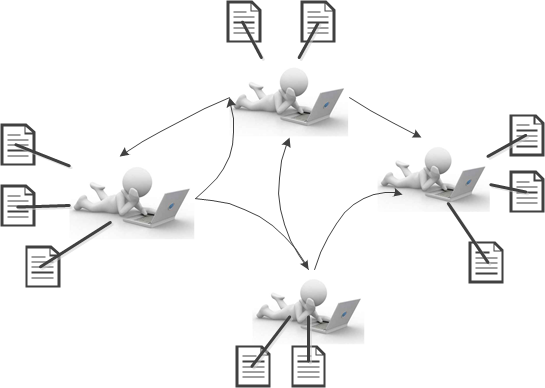
\includegraphics[height=200pt]{socialmedia.png}
\caption{形形色色的中英文社交媒体}
\label{socialmedia}
\end{figure}

社交媒体的迅速普及与壮大,使得它在政治、经济、教育、社会等多方面发挥着越来越重要的作用。例如,2008年的美国总统大选,奥巴马团队利用Facebook、Twitter等社交媒体,发布大量与竞选政策相关的信息向选民阐述,激发了青年人的小额捐款与投票,最终赢得美国大选,成为社交媒体的最大受益者。经济方面,由于用户在其社交媒体中发布大量的个人信息,使得社交媒体所在公司能够借助人工智能的方法对用户发布的内容进行分析,找到用户的兴趣爱好,以此进行广告投送。教育方面,许多科研工作者在其个人的社交媒体账户中发布与其科研课题相关的最新研究进展与相关资料,帮助其他从事相同研究或相近研究的人员迅速把握最新的研究动态。另外,由于社交媒体巨大的影响力,使得许多公益活动借助这个平台展开,例如,2011年初的“随手拍照解救乞讨儿童”运动\footnote{\url{http://weibo.com/jiejiuqier}},解救了不少走失儿童。同时社交媒体也作为公共平台,帮助老百姓对政府进行舆论监督,如“郭美美”\footnote{\url{http://zh.wikipedia.org/wiki/\%E9\%83\%AD\%E7\%BE\%8E\%E7\%BE\%8E\%E4\%BA\%8B\%E4\%BB\%B6}}、“表叔”\footnote{\url{http://baike.baidu.com/view/2172140.htm}},“房姐”\footnote{\url{http://zh.wikipedia.org/wiki/\%E9\%BE\%9A\%E7\%88\%B1\%E7\%88\%B1\%E8\%85\%90\%E8\%B4\%A5\%E6\%A1\%88}}事件等等。

就如社会会随着网络而演化,无论对个人还是商业组织,社交数据也逐渐变得越来越重要。Web 2.0时代的到来,更是由于广泛的用户参与而使得用户产生内容(user-generated content (UGC))成指数级的爆炸式增长,并且更庞大和复杂。近年来,情感分析(或者观点挖掘,sentiment analysis,opinion mining)研究逐渐发展成为介于自然语言处理(Natural Language Processing (NLP)) )与自然语言理解(natural language understanding(NLU))之间的一个独立领域。不像其他的自然语言处理任务(文摘或文本分类),观点挖掘主要处理与自然语言概念相关的语义信息和情感信息的推理而不需要对给定文本的深度分析\upcite{cambria2014jumping}。

在人类全部数字化数据中,仅有非常小的一部分(约占总数据量 的 1\%)数值型数据得到了深入分析和挖掘(如回归、分类、聚类),大型互联网企业对网页索引、社交数据等半结构化数据进行了浅层分
析(如排序)。占总量近 60\%的语音、图片、视频等非结构化数据还难以进行有效的分析\upcite{whitepaper2014}。目前常见的社交媒体数据挖掘应用有:一是基于用户个人信息、行为、位置、微博等数据而进行的个性化推荐、交叉推荐、品牌监测等营销类大数据应用,被互联网广告、电子商务、微博、视频、相亲等公司普遍采用。第二,公共服务类大数据应用,即不以盈利为目的、侧重于为社会公众提供服务的大数据应用。典型案例如谷歌开发的流感、登革热 等流行病预测应用能够比官方机构提前一周发现疫情爆发状况。国内也有搜索引擎公司提供诸如春运客流分析、失踪儿童搜寻的公益大数据服务。三是积极借助外部数据,主要是互联网数据,来实现相关应用。例如,金融机构通过收集互联网用户的微博数据、社交数据、历史交 易数据来评估用户的信用等级;证券分析机构通过整合新闻、股票论 坛、公司公告、行业研究报告、交易数据、行情数据、报单数据等, 试图分析和挖掘各种事件和因素对股市和股票价格走向的影响;监管机构将社交数据、网络新闻数据、网页数据等与监管机构的数据库对接,通过比对结果进行风险提示,提醒监管机构及时采取行动;零售 企业通过互联网用户数据分析商品销售趋势、用户偏好等等。一些服务商拥有海量用户数据的大型互联网企业,主要以SaaS形式为用户提供大数据服务,服务背后以自有社交媒体大数据资源为支撑。典型的服务如如谷歌Facebook的的自助式广告下单服务系统、Twitter 基于实时搜索数据的产品满意度分析等。国内百度推出的大数据营销服务 “司南”就属于此类。美国政府积极推动社交媒体数据公开,已开放37万个数据集,其中社交媒体数据集,同时,美国政府也是社交数据的积极使用者,2013 年曝光的棱镜门事件显示出美国国家安全部门在使用社交媒体数据应用的强大实力,其应用范围之广、水平之高、规模之大都远远超过人们的想象。2012-2013 年间美国国家安全局 (NSA)、联邦调查局(FBI)及中央情报局(CIA)等联邦政府机构大量使用Facebook,Google,Twitter等公司的数据对全球进行监控引起全世界的关注。随着应用的深入, 美国政府对大数据带来的负面影响也更加重视,白宫2014年5月发 布的《大数据:抓住机遇,守护价值》报告中提醒,在发挥正面价值的同时,应该警惕对大数据应用对隐私、公平等长远价值带来的负面影响\footnote{来源:\url{http://www.whitehouse.gov/sites/default/files/docs/big_data_privacy_report_may_1_2014.pdf}}。
我国社交媒体发展的宏观政策环境不断完善。2012年以来,科技部、发改委、工信部等部委在科技和产业化专项陆续支持了一批大数据相关项目,在推进技术研发方面取得了积极效果。2013年6月工信部发布的《电信和互联网用户个人信息保护规定》,根据《全国人民代表大会常务委员会关于加强网络信息保护的决定》,进一步界定了个人信息的范围,提出了个人信息的收集和使用规则、安全保障等要求,为大数据应用中的个人信息保护设立了法律法规屏障。2014 年《政府工作报告》明确提出,“以创新支撑和引领经济结构优化升级;设立新兴产业创业创新平台”,在新一代移动通信、集成电路、大数据等方面赶超先进,引领未来产业发展。近几年在互联网产业及金融、电信信息化快速发展的带动下,我国社交媒体数据资源总量有了快速增长,已达到全球的13\%。

那么什么是社交媒体,维基百科中给出了定义:\textbf{社交媒体就是一种人们在网络中交流的虚拟(社区)平台,在这个平台上人们创建、分享、交换信息和想法}\upcite{ahlqvist2008social}。从定义中我们可以看出,社交媒体是以互联网的思想和技术为基础的一项应用,用户可以借此进行内容创作、情感交流与信息分享。

目前,社交媒体的信息能够以多种不同的形式来呈现,包括文本、图像、音乐和视频等。国外流行的社交媒体包括了Twitter\footnote{\url{https://twitter.com/}}、Facebook\footnote{\url{https://www.facebook.com/}}、Youtube\footnote{\url{http://www.youtube.com/}}、Blogger\footnote{\url{http://www.blogger.com/}}、Flicker\footnote{\url{http://www.flickr.com/}}、Wikipedia\footnote{\url{http://www.wikipedia.org/}}、Google+\footnote{\url{https://plus.google.com/}}等;国内则包括了新浪微博\footnote{\url{http://weibo.com}}、腾讯微博\footnote{\url{http://t.qq.com/}}、人人网\footnote{\url{http://www.renren.com/}}、开心网\footnote{\url{http://www.kaixin001.com/}}、豆瓣\footnote{\url{http://www.douban.com}}、微信\footnote{\url{http://weixin.qq.com/}}、优酷\footnote{\url{http://www.youku.com/}}等等。

大部分社交媒体平台都是通过人与人之间的关系形成的社交网络聚合在一起。Kaplan和Haenlein将社交媒体主要分成六种类型\upcite{kaplan2010users}:
  \begin{enumerate}
  \item  \textbf{协同合作项目(Collaborative Projects)} 例如,维基百科(wikipedia)。
  \item   \textbf{博客和微博(Blogs and Microblogs)} 例如,Twitter和新浪微博。
   \item  \textbf{内容社区( Content Communities)} 例如,Youtube和优酷。
  \item  \textbf{社交网络网站( Social Networking Sites)} 例如,Facebook和人人网。
 \item  \textbf{虚拟的游戏世界( Virtual Game Worlds)} 例如,魔兽世界(World of Warcraft\footnote{\url{http://us.battle.net/wow/en/}})。
  \item  \textbf{虚拟社会世界( Virtual Social Worlds)} 例如,第二人生(Second Life\footnote{\url{http://secondlife.com}})。
  \end{enumerate}  
但是随着社交媒体的发展,不同类型之间的界限已经越来越模糊。Shi等人就认为Twitter是一种博客和社交网络网站结合的社交媒体\upcite{shi2011content}。

传统媒体如,报纸、电视、电影等,需要大量资源来发布信息。因此,在文章发表之前需要经过多次修改。而社交媒体发布消息相对廉价和方便,任何人都能够参与其中。但社交媒体与传统媒体也存在着共性,即消息能传播到或多或少的听众,例如,不论是博客还是电视,他们可能没有听众,但也有可能拥有成千上万的听众。

根据维基百科\footnote{\url{http://en.wikipedia.org/wiki/Social_media}},社交媒体与传统媒体的区别可以总结如下:
  \begin{enumerate}
    \item  \textbf{质量(Quality)} 传统的媒体发布消息是经过专业的编辑,质量相对较高。而社交媒体因为发布消息的门槛较低,编辑者编辑消息的水平差异较大,使得社交媒体中的消息质量参差不齐\upcite{agichtein2008finding}。
   \item  \textbf{传播性(Reach)} 虽然传统媒体与社交媒体都可以广播消息,不过两者信息传播的结构是不一样的。前者采用中央集权式的组织结构、生产、销售方式,后者通常呈现扁平化、无阶层、依照多元生产或使用的需求方式。
 \item  \textbf{使用性(Accessibility)} 一般使用传统媒体的用户大部分是政府和商业公司,而社交媒体的用户则可以是社会大众。
 \item  \textbf{可用性(Usability)} 传统媒体需要专业人士编辑后发布消息,而社交媒体只要具有一定资讯素养的用户就可随意发布消息。
\item  \textbf{及时性(Immediacy)} 一般而言,根据节目内容的规模,传统媒体常有几天、几周、几个月的制作时间;而社交媒体由于偏好发布较小的内容,通常制作时间只需要几小时、几分钟,甚至几秒钟而已。
\item  \textbf{固定性(Permanence)}  传统媒体的消息一旦发布,几乎很难修改,而社交媒体则常常随时随地的更新变化。
  \end{enumerate}  
  
由于社交媒体的迅速发展与参与用户的数目巨大,因此社交媒体中可挖掘的信息十分丰富,应用前景也十分广泛。但是信息量的庞大规模使得手工分析其中的内容变得十分困难,因此本文从信息自动化处理的角度对社交媒体的信息进行处理与挖掘,试图为社交媒体的相关应用提供帮助。

当然社交媒体与传统媒体存在显著的差异,其自身有不同的特点,如何分析其特点为自动化信息处理服务是我们关注的问题。另外,社交媒体的平台多种多样,基于平台使用的广泛性和代表性,再加上数据的公开性,我们选择Twitter作为我们的研究对象\footnote{本文作者十分感谢在英国爱丁堡大学留学期间,Miles Osborne教授提供相关Twitter数据进行本课题研究。},对其进行深入的分析与研究。

\subsection{Twitter}
社交媒体中最具代表性的应用莫过于微博,它是一种用户可以通过及时通讯、手机、电子邮件、网页等方式发布个人状态的消息交流平台。其中Twitter是最具代表性的微博工具,自2006年3月Twitter诞生之日起,截至2012年3月,Twitter 共有5亿注册用户,这些用户每天会发布约3.4亿条tweet(推文)\footnote{\url{http://techcrunch.com/2012/07/30/analyst-twitter-passed-500m\\-users-in-june-2012-140m-of-them-in-us-jakarta-biggest-tweeting-city/}},并且Twitter每天要接收16亿次检索查询\footnote{\url{https://blog.twitter.com/2011/engineering-behind-twitter's-new-search-exper}}。

有许多用户发布的Twitter消息创造了历史。一个早期的案例是2008年4月一位美国学生通过Twitter通知好友,他在埃及马哈拉被反政府抗议者扣押,后来这条消息迅速转发,随着巨大的舆论压力,他在第二天就被释放\footnote{\url{https://twitter.com/jamesbuck/status/786571964}}。2009年1月全美航空的飞机迫降哈德逊河,目击者拍摄了一张乘客们在机翼上等待救援的照片,随后该条消息被迅速转发,从此确立了Twitter实时新闻的传播工具地位\footnote{\url{http://twitpic.com/135xa}}。2009年5月12日航天员蒂莫西·克里莫(Timothy Creamer)第一次从太空发布了tweet \footnote{\url{https://twitter.com/Astro_TJ/status/8062317551}}。

另外,还有一些与Twitter的有关事件确立了Twitter在人类生活中的重要地位。例如,2010年4月美国国会图书馆宣布收录所有的公共Twitter消息\footnote{\url{http://www.loc.gov/today/pr/2010/10-081.html}}。2012年12月教皇本笃十六世开通Twitter账号“@Pontifex”\footnote{\url{https://twitter.com/Pontifex}},成为首位使用Twitter的教皇,他的继任者方济各(Pope Francis)继续维护着这个账号。2013年1月贾斯汀·比伯(Justin Bieber)超越Lady Gaga,成为Twitter粉丝最多的用户,目前的粉丝数超过4400万\footnote{\url{https://twitter.com/justinbieber}}。

以上种种事件都说明Twitter作为社交媒体的代表具有巨大的影响力,再加上数据的公开性,因此本文以Twitter作为研究对象,进行详细的社交媒体分析与研究。当然Twitter作为社交媒体的代表也有它自身的属性,下面我们从Twitter的主要功能进行详细的介绍。

图~\ref{Twitter}给出了本文作者Twitter主页的示意图。我们可以看到主页中有许多不同的人发布的tweet(消息),tweet的话题可以从日常生活,新闻,到其他任何感兴趣的事情,每个tweet限制在140个字符以内。140个字符的原因是由于Twitter在最开始设计的时候是基于短信平台,后来随着不断的发展,许多其他的客户端开始投入应用,包括网页和桌面客户端等,但是这个tweet的长度限制还是保留了下来,并且还被重新作为一个功能叙述。这种文本长度的限制反而促进了Twitter用户编辑的简便和交流的方便,Twitter的创意总监Zinko曾认为“creativity comes from constraint”就是一个很好的佐证\upcite{zinko2009biz}。

\begin{figure}[htp]
\centering
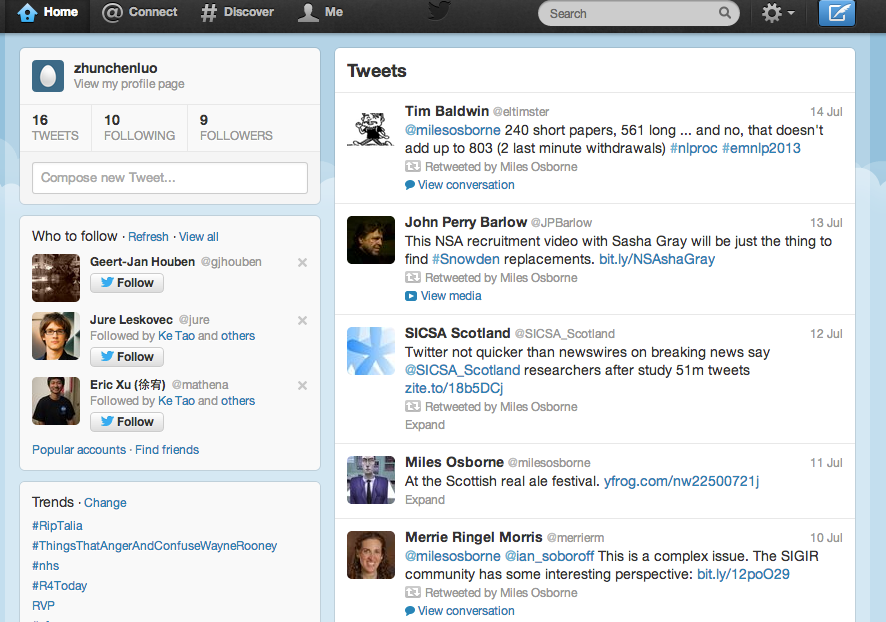
\includegraphics[height=280pt]{Twitter.png}
\caption{Twitter示意图}
\label{Twitter}
\end{figure}

随着越来越多的用户使用Twitter,且其中许多人都投入了巨大的热情和精力,使得Twitter成为了一个活跃的网络社区,有着自己一套独特的交友方式和评价体系。Twitter结合了已有的社交网络和博客的元素\upcite{ellison2007social,marlow2005structural},但也存在着明显的区别:
   \begin{enumerate}
    \item 类似于社交网络,Twitter用户也通过一定的社会关系或兴趣爱好建立联系形成社交网络,但是这种用户之间的联系不是双向的而是单向的。用户可以关注其他用户(“follow”),订阅对方发布的tweet,而对方并不需要关注该用户。
    \item 类似于博客,Twitter用户的主页中按时间顺序(默认设置是由近至远)展示他所发布的tweet,但并不允许其他人直接对每个tweet进行评论\footnote{这个明显区别于新浪微博的评论功能。}。
     \item Twitter用户的隐私设置一般是公开的,但用户也可以设置成保护状态,使得其他用户无法看到。
  \end{enumerate}  

Twitter最主要的功能就是当用户注册以后,一个其关注对象发布的tweet流将按时间倒序展示出来(见图~\ref{Twitter})。每个用户都有自己不同的原则关注其他用户(见图~\ref{Twitter}中“FOLLOWING”),例如有些用户关注了成千上万的用户,有些用户只关注了几个个人熟悉的用户,有些关注名人,有些关注了日常生活不认识但发布内容感兴趣的用户。

至于用户在Twitter中可以交流的工具,不仅有Twitter网站本身,还有许多第三方应用,包括手机应用,桌面客服端等,这些不仅帮助用户发布tweet和交流,有时还提供其他一些功能,如帮助用户发现热门话题,提供感兴趣的其他用户进行关注等。这些应用的大量设计与开发主要归功于Twitter开放自身的API\upcite{o2011twitter},使得研发人员可以利用Twitter数据,设计相关应用。

由于tweet~140个字符的限制,使得Twitter用户渐渐采用了一些独特方式表示一些功能。例如当用户发布tweet想涉及某人时,他们将“@”符号与其涉及对象的用户名结合在一起,如见图~\ref{Twitter}中的“@milesosborne”。这是一种特殊的约定,起源于以前的即时聊天系统,这个方式目前在Twitter中有两个功能:
   \begin{enumerate}
    \item 直接发消息到某人作为回复(reply),Honeycutt和Herring将其成为“地址性(addressivity)”\upcite{honey2009beyond}。
    \item 在发布tweet时涉及某人,例如,tweet:\emph{I saw @oprah's show today},以引起对方的注意。
  \end{enumerate}  

Twitter中另外一个重要的约定方式就是“标签(hashtag)”,主要表示tweet的话题,它由符号“\#”与关键词组合而成。这种方式类似与网页中“社会标签(tag)”,方便标注主题以此进行分类或检索\upcite{golder2006usage}。 另外,hashtag可能起源于以前程序员之间使用特定的词汇与标点符合,例如“\$”和“\ * ”表示各种变量与指针或使用“\#”符合识别HTML锚点的历史。

最后Twitter中最特别的一个功能就是转发(Retweet),即重新发布其他人发布过的tweet。它不同于“@username”和hashtag功能表示单一,转发的表示有许多不同的形式,最常用的形式就是拷贝其他人的tweet,然后在这个tweet的前面添加“RT”和来源地址(@username),例如:
 \begin{description}
    \item \textbf{A:} \emph{Hello world!}
    \item \textbf{B:} \emph{RT @A: Hello world!}
  \end{description}  
B就是转发来自A的tweet。当然实际的转发方式可能远比上面的例子复杂。目前除了Twitter提供了一个自动的转发按钮便于用户转发,其他的人工添加符号表示转发的方式还有很多,例如,“RT”、“rt”,“via@username”等等。由于tweet~140个字符的限制,用户转发时可能只截取原始tweet部分内容,还有些用户在转发的tweet的文本前面加上一段自己的评论,甚至有些用户并不是完全复制原始tweet的内容,有些进行重新编辑然后再发布。以上种种使得tweet在转发时可能在内容上有一定的变化,转发方式的不一致都使得转发的识别变得困难,影响了Twitter中信息传播研究的信息跟踪。

但是Twitter的转发功能也为相关研究提供了机遇,如tweet被转发的次数可以反映tweet所涉及话题的热度,另外,转发的内容一般都是高质量的消息,最后转发还反映了转发者对被转发者发布消息的肯定态度。

毫无疑问,Twitter使用的广泛性,以及用户通过这个平台发布大量的消息,使得从Twitter中获取相关信息变得十分有意义。但是数据量的巨大也造成手工方式的获取变得困难,因此本文通过自动化的方式从海量的Twitter数据中获取相关信息为其它Twitter应用服务。另外,Twitter是一定的关系建立的社交网络,通过“@username”进行交流,利用hashtag标注tweet主题,使用转发传播信息都使得Twitter成为一个研究者分析社会热点,理解人类交流方式,解析人物关系网等情况的重要数据。这些功能与方式都使得Twitter具有其自身独特的特点,本文将对其特点进行深入的探讨。

\section{研究问题}
\label{point}
随着以Twitter,Facebook、新浪微博为代表的社交媒体迅速发展,如何帮助人们利用平台更好地交流,并且在这些社交媒体中发现有意义的信息变得越来越重要。而信息检索技术是满足以上需求的重要技术手段。信息检索是在文档集合中,找到与给定话题相关的客观文本或主观文本。它能够帮助人们在海量的社交媒体信息中,快速找到相关内容,帮助有意义的信息发现,以此满足人们的需求,方便人际之间的交流。另外,以Twitter为代表的社交媒体的一个显著特点,就是信息的传播性。人们通过转发分享新闻与观点,加速信息的流动、扩大信息传播的范围。另外,Twitter中已有的研究发现,转发的信息往往意味着高质量的信息\upcite{hong2011predicting},这是基于人们在Twitter传播行为上的一个基本假设:当人们认为一个tweet非常重要且值得和大家分享此信息时,他们将通过转发传播这个tweet。因此研究社交媒体中信息传播的内在规律变得十分重要,且可以帮助在Twitter中检索高质量的信息。

但是Twitter中的信息检索与传播分析任务也存在着挑战。由于Twitter客户端使用的多样性,如大量使用移动平台,以及tweet文本本身140个字符的限制,造成tweet文本与其他文本(如新闻)编辑质量与风格的巨大差异。同时移动平台的广泛使用,使得Twitter中信息传播速度更快,范围更广。再加上Twitter用户参与的低门槛性,使得信息在Twitter中的传播不像以往媒体(如报纸)的新闻传播,会对信息的正确性进行层层验证,这就造成了Twitter中信息传播的随意性,使得信息的质量难以保证。因此本文主要从两个科学问题来思考与研究Twitter,以此帮助Twitter中的信息检索与传播分析:
    \begin{enumerate}
    \item \textbf{人们在Twitter中如何用自然语言描述话题和表达观点?}
    \item \textbf{以Twitter为代表的社交媒体有何新特点?如何利用这些特点帮助获取信息和对信息进行传播分析?}
    \end{enumerate}  

第一个问题的研究主要是从自然语言处理的角度分析人们在社交媒体上如何组织语言来描述客观话题和表达主观观点。显然Twitter参与的低门槛特点使得大量的用户参与其中,由于参与者编辑文本的水平参差不齐,编辑的内容与目的也多种多样,另外,再加上tweet本身的字符限制都使得Twitter中的文本呈现低质量、噪音大的短文本特点,这给传统的以正式文本(如新闻)为处理对象的自然语言处理技术带来了挑战。因此深入地研究Twitter文本的特点,对于解决Twitter中的信息检索与传播分析任务变得十分重要,并且分析Twitter中文本的特点也能够帮助其他以语言为基础的Twitter应用,如Twitter中的事件发现、观点挖掘等等。

第二个问题的研究主要是分析Twitter作为新型媒体的特点,从中发现一些规律和有价值的信息帮助Twitter中信息检索与传播分析问题的解决。显然Twitter中无论是tweet本身还是tweet的用户都呈现了一些新的特点。比如,tweet中包含hashtag,以此可以作为tweet的内容主题。tweet中也包含大量的链接,这些链接与tweet中描述链接的文本存在什么样的关系?另外,每个tweet都有作者,Twitter的一个显著特点就是用户信息的公开化,包括用户的朋友关系,发布信息的历史,个人的属性信息等,如何发现这些用户信息的普遍规律与内在价值,以此帮助Twitter中的信息检索与传播分析任务是本文研究的主要问题,当然社交媒体的新特点研究同样也能帮助Twitter中其他任务的解决,如用户推荐等。

\section{相关研究}
无论是Twitter中的信息检索还是传播分析,对tweet文本的理解都是其中一个重要的环节。但是tweet文本的短小与大量的噪音文本(存在着许多缩写词、错别字等等)都造成自然语言处理技术在Twitter上的应用存在着新的挑战,我们在本节将介绍自然语言处理技术在tweet文本处理上的相关工作。另外,Twitter上信息检索的研究也离不开以往传统信息检索技术的借鉴与应用,我们主要利用tweet的文本特征与社交媒体的特征帮助Twitter中的信息检索,而这些特征如何有效地整合到检索模型中是需要考虑的问题,因此本节将详细介绍基于机器学习的信息检索技术。最后本节还将介绍已有的Twitter中的传播分析工作,以此为本文具体的传播分析任务的解决提供帮助。

这里要强调的是,本文的相关工作分析主要从整体相关工作和局部相关工作进行阐述。本章的相关研究主要介绍的是整体的相关工作,因为这些研究成果可以为本文所研究的具体任务提供思想借鉴和技术支持。以后各个章节中的相关工作则会具体地分析已有的类似工作,以及研究成果。

我们从整体上介绍了三个相关研究,包括Twitter与自然语言处理(见~\ref{rel1}),主要介绍目前已有的自然语言处理技术在Twitter中的研究成果,以此帮助本文的关于tweet的文本分析;信息检索与机器学习(见~\ref{rel2}),主要介绍目前机器学习技术在信息检索中的应用,以此为解决本文的具体Twitter信息检索和传播分析任务提供问题解决框架;Twitter中的传播分析(见~\ref{rel3}),主要介绍目前已有的关于Twitter转发的研究成果,为本文Twitter传播分析的具体任务提供借鉴。

\subsection{Twitter与自然语言处理}
\label{rel1}
随着以Twitter为代表的社交媒体的广泛使用,自然语言处理技术在Twitter的文本处理中得到广泛应用,但是研究者发现Twitter的文本明显区别于以往的很多文本类型。Eisenstein将这种文本类型称为\emph{坏语言(bad language)}:文本“无视”我们以前期望的词汇、拼写和语法\upcite{eisenstein2013bad}。

研究人员发现最先进的自然语言处理技术在Twitter的文本应用中都显著差于其他文本。在自动地词性标注测试中,Stanford tagger在Wall Street Journal语料上的正确率可以达到97\%\upcite{toutanova2003feature},而tweet的文本处理仅仅只有85\%\upcite{gimpel2010part,owoputi2013improved}。利用CoNLL数据训练的Stanford命名实体识别器,对CoNLL测试语料进行实体识别,F1值可以达到86\%\upcite{finkel2005incorporating},而在Twitter的文本中仅仅只有44\%的F1值\upcite{ritter2011named}。另外,Foster等人也对语法分析效果进行分析,发现最先进的语法分析器在Twitter的文本应用中,正确率下降约15\%\upcite{foster2011news}。

为了解决自然语言处理技术在Twitter中所遇到的挑战,研究人员主要从两个方面进行了相关研究:
\begin{enumerate}
\item \textbf{文本的正常化(Normalization)},即把坏语言变成好的语言,以其适合于传统文本的自然语言处理技术。Han和Baldwin开发了一个分类器,能够识别“非正常(ill-formed)”的词,然后利用基于形态音位(morphophonemic)相似的方法将其转换为正确的词\upcite{han2011lexical,han2013lexical},Han等人还提出了一种构造词典的方法,简单替换词的变形(例如tomorrow替换tmrw),这种方法结合词语的上下文评估各种变换的可能性\upcite{han2012automatically},但Liu等人提出一种没有明确分类的方法,进行词的正常化\upcite{liu2011insertion}。另外,Liu等人提出了一种基于图模型的方法同时解决tweet中命名实体识别和tweet文本正常化的方法\upcite{liu2012joint} 。Liu等人设计一个正常化认知驱动系统解决Twitter中文本的正常化问题\upcite{liu2012broad},该系统整合人们对于“非正常(ill-formed)”词的各种认知角度,包括字符转换、视觉感知、字符串和语音相似等等。最近Hany和Menezes提出了一种无监督学习的方法对Twitter中的文本进行正常化,他们在大量tweet文本中构造n元词串,以此构造语境相似的二部图,然后利用Random Walks算法发现“非正常(ill-formed)”词与正常词的对应关系\upcite{Hassan2013}。以上所有的方法都在一定程度上解决了Twitter中文本正常化的问题。

\item \textbf{领域化(Domain adaptation)} 与其让Twitter的文本适应以前的自然语言处理技术,不如改变这些技术适应Twitter文本。一系列的工作从领域化的角度出发进行了相关研究。这些工作包括适合Twitter文本的自动词性标注器\upcite{gimpel2010part,owoputi2013improved},自动命名实体识别的方法\upcite{finin2010annotating,ritter2011named,liu2011recognizing,li2012twiner,liu2012joint,liu2013named,liu2012two},语法分析器\upcite{foster2011news},对话模型\upcite{ritter2010unsupervised},自动摘要\upcite{sharifi2010summarizing,chakrabarti2011event,takamura2011summarizing,weng2011imass,harabagiu2011relevance,Ren:2013:PTT:2484028.2484052,shen2013participant,judd2013better,chang2013towards}等等。这些工作采用各种方法,使其能够很好地适应Twitter文本的特点,具体为:
\subitem \textbf{预处理(preprocessing)} 减少词语中某些重复的字符(经常有些词用重复的字符表达感情\upcite{brody2011cooooooooooooooollllllllllllll}),去掉hashtag、链接、提交(@username)等等;
\subitem  \textbf{标注新数据(new labeled data)} 根据任务在Twitter中标注部分数据\upcite{finin2010annotating,ritter2011named},以此进行有监督学习;
\subitem \textbf{自定义标注标准(new annotation schemes)} 定义适合Twitter的标注标注,如词性标注中对hashtag、链接、提交(@username)等定制特定的标注类型\upcite{gimpel2010part,owoputi2013improved};
\subitem \textbf{“	远端”监督(distant supervision)} 通过一定的规则,构造大量粗糙的训练数据帮助Twitter的文本机器学习模型训练,然后应用到具体的任务中\upcite{ritter2011named}。
\end{enumerate}

毫无疑问,tweet文本的特殊性使得传统自然语言技术在Twitter上的应用充满挑战,我们将利用以上所涉及到的方法、思想或已有的开发工具,按照信息检索任务和传播分析任务的具体需求,设计对应的tweet文本自然语言处理方法,开发有效的文本特征,提高Twitter中的信息检索效果与传播分析的准确性。

\subsection{信息检索与机器学习}
\label{rel2}
Twitter中的信息检索是本文的一个重要研究任务,由于tweet文本的特点和丰富的社交媒体属性使得Twitter中的信息检索不同于以往的信息检索任务(如图书馆文档检索)。在Twitter检索任务中需要考虑因素很多,如tweet用户的信息等。传统的检索模型在构造排序函数的时候往往只需要考虑不多的因素,如查询词在文档的频率、位置等,因此可以手工构造这些函数对文档排序,但是 Twitter中的检索需要考虑的因素相当多,造成手工构造排序函数变得复杂,但是基于机器学习的排序模型可以通过训练数据自动构造排序函数,因此这里我们详细介绍基于机器学习的信息检索模型。

信息检索与机器学习领域有很多研究的重叠,上世纪60年代提出的相关反馈就是一个简单的机器学习算法,它构建一个分类器区分相关文档和非相关文档,以此作为用户关于初始排序中文档重要性的反馈\upcite{rocchio1971relevance}。到了80、90年代,研究人员开始使用机器学习方法来基于用户反馈学习排序算法。但是,许多机器学习算法在信息检索上的应用都受到训练数据规模较小的影响,如果系统要对每个查询构造分类器,基本上是不现实的。

但进入21世纪,随着网络搜索引擎的出现,从用户交互中积累了海量的查询日志,潜在的训练数据的规模非常庞大。借此基于点击流数据的排序学习算法被提出\upcite{joachims2002optimizing,xue2004optimizing,joachims2005accurately,radlinski2005query,agichtein2006improving,agichtein2006learning,radlinski2007active,bao2007optimizing}。由于对于每个查询中文档的相关性判断非常稀疏,但是有一定数量文档在网络搜索引擎的检索返回结果中被用户点击浏览,这些行为可以隐性地认为是用户对文档相关性的判定。例如,如果一个用户在一个查询的排序中点击了第三个文档而不是前面两个,那么可以假设第三个文档应该在下次排序中获得较高的排序位置。

在排序学习模型中,最著名的排序函数莫过于基于支持向量机(SVM)的方法,通常被称为Ranking SVM。 它的输入是针对一组查询的偏序排序信息的训练集合:
$$(q_1,r_1),(q_2,r_2),...,(q_n,r_n)$$
其中$q_i$是一个查询,$r_i$是所需排序的文档关于查询的部分排序信息或相关性级别。这意味着如果文档$d_a$应该比$d_b$排序更高,那么$(d_a,d_b)\in r_i$。这些排序信息可以通过点击流数据获得,然后训练排序模型。相关的研究从排序学习的数据\upcite{duh2008learning,aslam2009document,qin2010letor,xu2010improving}、排序学习模型\upcite{burges2005learning,cao2006adapting,xu2007adarank,quoc2007learning}和评估学习效果\upcite{xu2008directly,valizadegan2009learning,wang2010learning,dai2011learning,chapelle2011future}三个方面展开。

本文将主要采取基于排序学习的机器学习算法,针对Twitter信息检索的具体问题,将tweet文本分析的结果和Twitter社交媒体的新特点转换成特征,整合到机器学习的模型框架中,帮助Twitter中各项检索任务的解决 。

\subsection{Twitter中的传播分析}
\label{rel3}
Twitter中一个重要的机制就是转发,即重新发布其他人发布过的tweet。这种简单的机制可以使得作者的全部粉丝看到转发的信息,使得信息迅速、广泛的传播。我们本节将介绍Twitter中已有的对于转发行为的研究,以此分析涉及影响转发行为的因素,包括tweet的文本内容与转发的关系,用户的属性如何决定其他人的转发;Twitter中信息的一般传播路径与规律。这些研究成果可以帮助本文具体的传播分析任务。

boyd等人\footnote{Danah Boyd因为家庭的原因一般使用小写拼写姓名,这里并不是拼写错误。}研究了Twitter中转发的各种类型以及转发的原因,他们分析了不同用户,用户属性,用户交流方式对于转发的影响,同时也分析了人们在Twitter中喜欢转发的内容\upcite{boyd2010tweet}。他们发现18\%的转发tweet包含hashtag,52\%的转发tweet包含链接,11\%的转发tweet包含连续的转发符号串(如,“RT @user1 RT @user2 ”),另外,9\%的转发tweet都包含回复原tweet作者的回复字符串(“@reply”)。这说明tweet文本中的hashtag,链接、回复、提交和转发符号都与tweet的转发存在着一定的对应关系。

Yang和Counts通过Twitter中的提及(“@username”)抽取了用户之间的关系,并在此基础上构造了用户关系的复杂网络。他们研究了信息在这个复杂网络上是如何传播的,包括信息传播的速度,规模,以及范围\upcite{yang2010understanding}。他们发现大约只有25\%的tweet是被信息作者的朋友转发,大部分是被粉丝但非朋友转发。这说明Twitter中用户形成的复杂网络,影响着人们的转发行为,因此信息在传播路径上具有一定的规律可循。

Macskassy和Michelson分析了一个月用户的Twitter数据,他们解释了各种信息传播的方式,尤其是转发的行为模式,他们发现tweet的内容是tweet被转发的决定因素,因此他们构建了基于内容的转发模型\upcite{macskassy2011people}。

Starbird等人对具体事件在Twitter上的传播进行了深入研究,他们分析了2011年埃及的政治事件,演示了这个事件的相关信息在Twitter上是如何生成,发展,传播的\upcite{starbird2012will}。

Comarela等人研究了影响用户回复或转发的因素,他们发现以前是否回复,发布信息的频率,信息的时效性,tweet的长度决定用户是否回复\upcite{comarela2012understanding}。

除了以上的工作,最新的研究还从不同角度对Twitter中的转发行为进行了深入的研究\upcite{kupavskii2013predicting,jenders2013analyzing,ahmed2013peek,bao2013popularity}。

综上所述,我们发现影响人们转发行为的因素主要包括tweet文本的内容、tweet文本的社交媒体属性(如,是否包含链接、hashtag、提及等)、tweet作者的用户属性,tweet作者的朋友圈子,当然以上的研究都是从宏观上大规模分析Twitter转发数据得出的研究结论。从微观的角度则可以考虑给定一个tweet,未来这个tweet是否会被转发,我们将在~\ref{rel_retweet}介绍相关工作。

虽然已有的Twitter转发研究从许多不同的角度进行了考虑,但是仍然有许多问题与因素被忽视,例如tweet的转发预测针对的一般是普遍tweet,并未细粒度的划分类型,本文我们将针对特定类型tweet进行转发研究。另外,目前的转发大多都是从tweet本身进行考虑,并未从受众的角度进行分析,本文将对tweet,作者、受众三个方面在转发过程中的相互关系进行探讨。



\section{研究内容与方法}

\subsection{本文研究内容}
本文的研究内容主要是围绕在给定话题的情况下,如何在Twitter中找到与话题相关的主客观tweet。主要利用tweet文本特点和社交媒体属性帮助Twitter中的信息检索。本文中Twitter的传播分析主要是从内容和受众两个方面进行考虑,如何在Twitter中发现会传播的观点和如何在Twitter中发现信息的传播者。同样也通过分析tweet文本特点和社交媒体特点帮助这两个问题的解决。参见图\ref{Research_Framwork}本文研究框架。

\begin{figure}[htp]
\centering
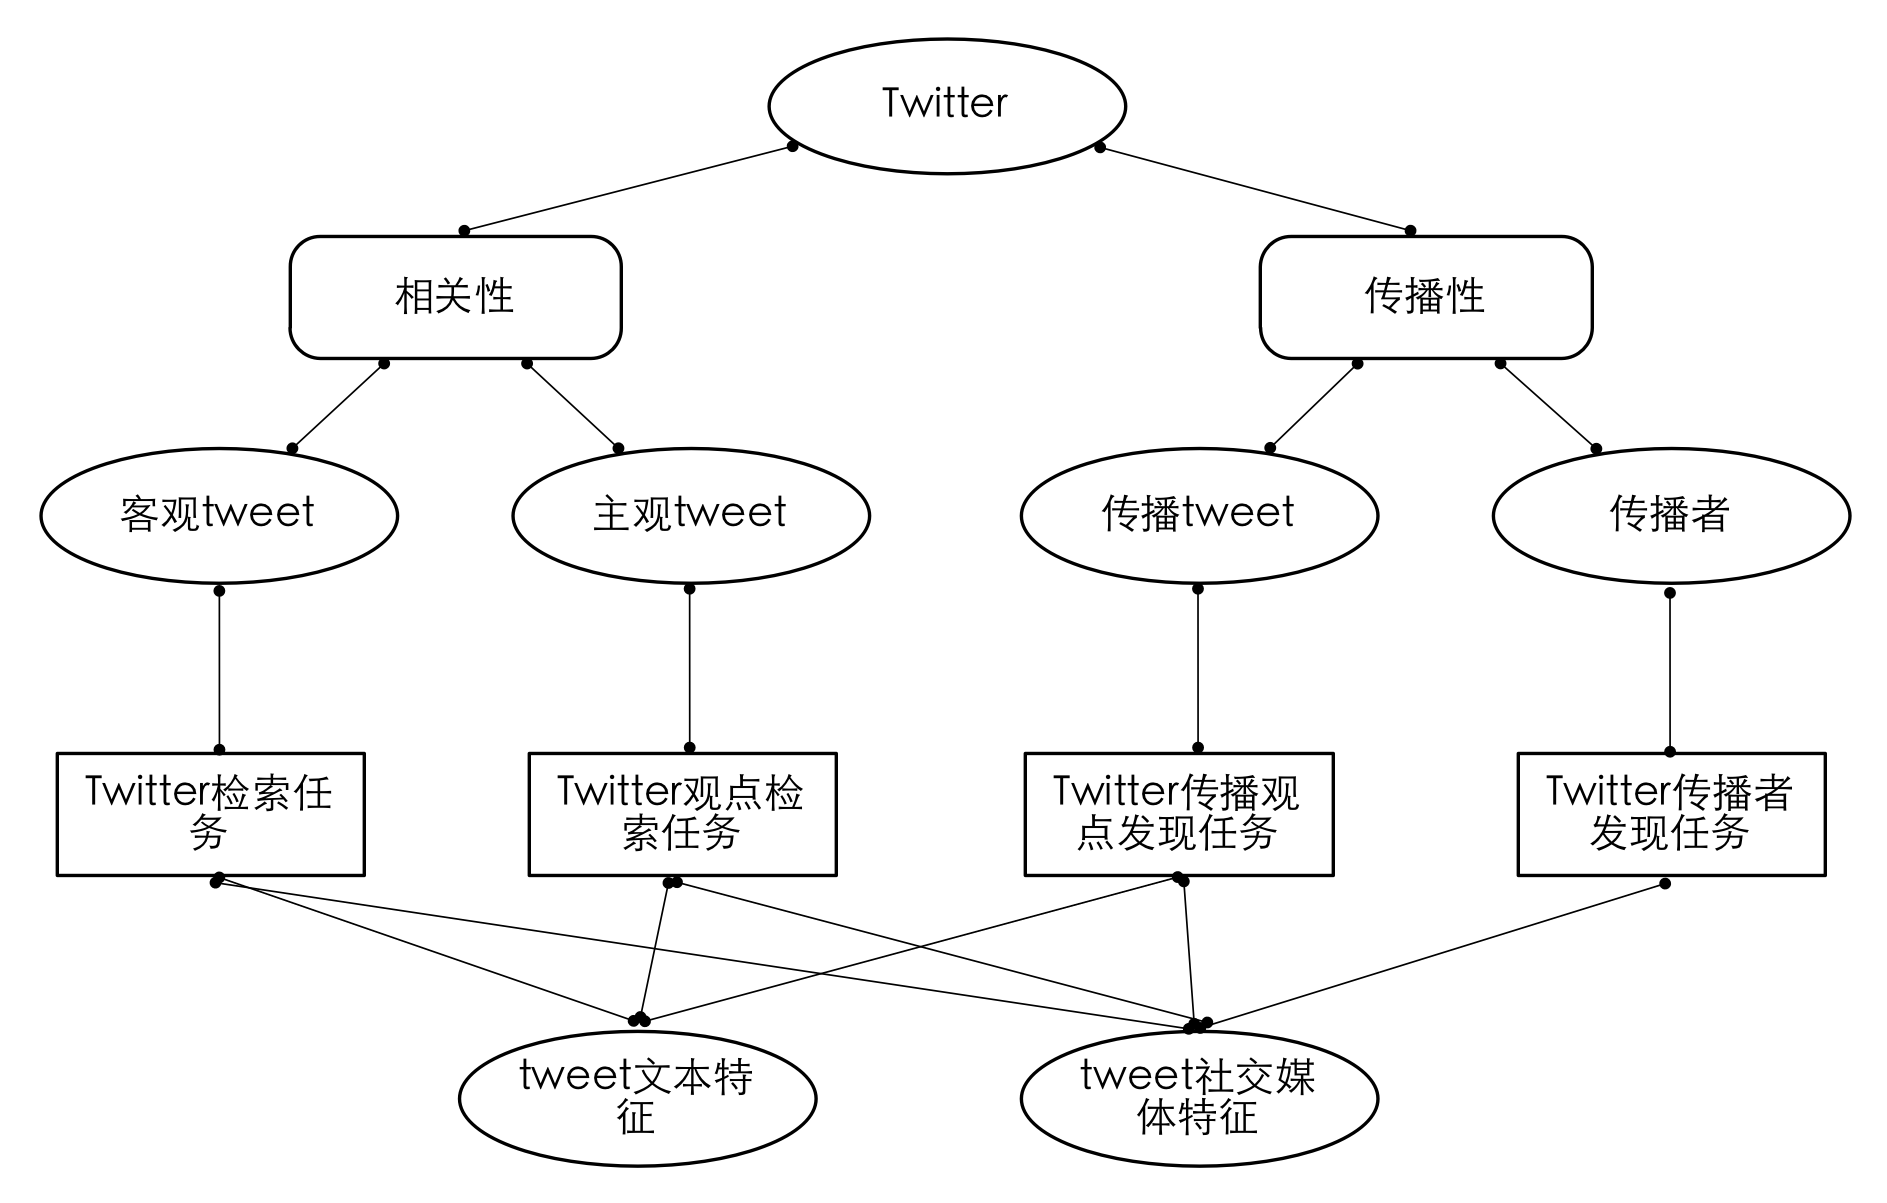
\includegraphics[height=250pt]{Research_Framwork.png}
\caption{本文研究框架}
\label{Research_Framwork}
\end{figure}

具体四个研究内容的定义如下:

\begin{enumerate}
\item \textbf{Twitter检索}:给定关键词,在Twitter中找到话题相关的tweet。通过文本的结构化信息(我们发现tweet文本呈现结构化特点)和社交媒体信息帮助提高Twitter检索,以此分析了人们在Twitter中是如何描述话题以及社交媒体特征与相关话题tweet的内在联系。
\item \textbf{Twitter观点检索}:给定关键词,在Twitter中找到话题相关且带观点的tweet。通过tweet观点化信息(基于结构化信息)和社交媒体信息帮助提高Twitter观点检索,以此分析了人们在Twitter中是如何表达观点以及社交媒体特征与Twitter中观点的内在联系。
\item \textbf{Twitter传播观点发现}:给定关键词,在Twitter中找到话题相关且带观点的tweet,并且这个tweet在未来会被转发。通过tweet观点化信息(基于结构化信息)和社交媒体信息帮助发现Twitter中传播观点,以此分析了人们在Twitter中是如何表达高质量的观点以及社交媒体特征与Twitter中传播观点的内在联系。
\item \textbf{Twitter传播观者发现}:给定tweet,发现tweet的粉丝中,谁会在未来传播这个tweet。通过社交媒体信息帮助发现Twitter中的信息传播者,以此分析了社交媒体特征与Twitter信息传播者的内在联系。
\end{enumerate}

总的来说,针对~\ref{point}的第一个问题,本文通过分析tweet文本的结构化信息和观点表达方式,找出规律与特点,将其利用到Twitter检索、观点检索、传播观点发现任务。
针对~\ref{point}的第二个问题,本文通过分析社交媒体的用户属性、社会网络结构、文本属性,发现用户之间、用户与tweet文本(主客观信息)、用户与传播行为、tweet文本与传播行为之间的内在联系,通过开发社交媒体特征,帮助解决Twitter检索、观点检索、传播观点发现和信息传播者发现任务。

\subsection{本文研究方法}
针对以上研究内容,本文基于自然语言处理技术和机器学习技术,深入分析Twitter中tweet的文本特点和社交媒体属性,解决Twitter中若干检索与传播分析问题。我们希望通过对Twitter中若干检索与传播分析问题的研究达到如下几个主要目标:
\begin{enumerate}
\item 认识以Twitter为代表的社交媒体的新特点,包括文本表现形式,用户属性,Twitter中信息的传播行为等等。
\item 传统的信息检索技术如何在新型的社交媒体中使用,重点研究基于机器学习的信息检索技术在Twitter中的应用。
\item 深入研究Twitter中观点检索问题,寻找人们在Twitter中表达观点的方式,以及其它相关因素。
\item 针对Twitter中tweet文本质量较低,以及质量评价问题,帮助人们进一步理解Twitter中高质量文本的评价问题。
\item 通过研究特定用户查询问题,找到Twitter中tweet、作者和粉丝之间的关系,帮助Twitter中传播分析的研究。
\end{enumerate}  

根据各个具体的研究内容,我们的具体研究方法为:

\begin{enumerate}
\item 针对Twitter中的信息检索问题,我们深入分析tweet中的文本特点,找到文本特定结构与社会属性之间的关系,开发文本结构特征,然后结合tweet的社交媒体特征(用户属性等),将其整合到机器学习的框架中,通过排序学习,提高Twitter中信息检索的效果。
\item 针对Twitter中的观点检索问题,首先对Twitter中的观点检索问题进行定义,构造测试数据集,然后分析Twitter中用户表达观点的文本特点以及Twitter中观点所对应的潜在用户属性,开发特征,利用排序学习,解决Twitter中如何找到观点的问题。
\item 针对Twitter观点检索中大量返回低质量观点的问题,从发现传播观点的角度提出了Twitter中高质量观点的客观评价指标,这个指标利用Twitter中高质量信息大量传播的特点,分析了Twitter传播观点发现的问题,利用tweet中如何判定是否转发的方法,tweet中文本是否包含观点以及tweet文本本身的语言质量帮助相关任务的解决。
\item  针对Twitter中信息传播者发现的问题,我们首先进行问题定义,构造数据集,分析信息传播者的特点,找到信息传播者与转发tweet、转发tweet作者之间的联系,设计相关特征,将其利用到机器学习框架中,解决信息传播者发现的问题。
\end{enumerate}  

\section{本文主要贡献}
本文主要围绕分析Twitter文本的特点与Twitter社交媒体属性展开,通过Twitter中的信息检索和传播分析任务,发现哪些因素能够帮助或影响检索效果的提高与传播分析的准确性。

在tweet文本分析方面,我们发现,虽然tweet是短文本,但是它具有结构化的特点。不同的tweet文本结构对应不同的属性和文本质量,通过挖掘tweet的文本结构信息能够帮助Twitter的信息检索。另外由于某些特定结构的tweet具有某种属性(如主观化),因此可以利用结构化的tweet收集大量的相关文本,构造情感词典帮助tweet主观化判定,提高观点检索的效果。

在Twitter社交媒体属性的分析方面,我们通过对tweet中是否包含链接、hashtag、提及等的研究,确定这些符号串或功能与Twitter信息检索的对应关系,因此帮助该任务的解决。我们还分析了tweet作者的属性,包括作者的粉丝数目、朋友数目、分组数目、兴趣爱好、圈子、活跃时间等等,试图发现这些因素与Twitter信息传播之间的内在联系。

在具体的Twitter信息检索任务中,我们从给定关键词找到主客观相关tweet的两个方面进行研究。获取客观tweet方面,我们开发了tweet文本的结构化特征和社交媒体特征,将其整合到基于排序学习的模型中,实验结果验证了我们的方法是有效的。获取主观tweet即Twitter中的观点检索是一个全新的工作,我们定义了这个问题,发布了关于研究这个问题的实验数据\footnote{下载地址:\url{http://sourceforge.net/p/ortwitter/wiki/Home/}},截止到2013年9月这个实验数据已经有40多个国家和地区超过200多个研究单位和个人下载,并且这个数据还被ICWSM会议推荐为官方的社交媒体研究数据\footnote{\url{http://www.icwsm.org/2013/datasets/datasets/}},针对Twitter中的观点检索我们也提出了我们的方法,主要是开发tweet的文本特征与社交媒体特征结合排序学习框架进行解决,同时我们也提出了一种基于无监督学习的tweet观点化评价的方法,目前有许多其它研究单位的工作围绕我们的Twitter观点检索工作展开\upcite{stajner2013automatic,kothari2013detecting,li2013exploiting,zhang2013personalized}。

在具体的Twitter传播分析任务中,我们从传播的内容和受众两个方面进行考虑,提出了Twitter中传播观点发现的新任务和信息传播者发现的新任务。Twitter中传播观点发现可以帮助我们解决tweet质量评价主观化的问题,由于以往的研究主要是围绕给定tweet,预测该tweet在未来是否会被转发,我们对这个问题进行了细粒度的研究,从观点化的tweet能否被转发的角度进行了探讨,通过开发tweet的文本特征和社交媒体特征解决传播观点发现的问题。Twitter信息传播者发现的问题,针对的是以往研究忽视“谁”会转发的问题,我们定义了这个问题,提出了解决这个问题的方法,发现兴趣与转发的历史信息是决定信息传播者的重要因素,同样我们也公布了研究这个问题的数据集\footnote{下载地址:\url{https://sourceforge.net/projects/retweeter/}},供以后科研人员继续使用。

以上所有的工作都通过论文的形式公开发表\upcite{luo2012improving,luo2012opinion,l2013Luo_POR,Luo:2013:RMF:2484028.2484158}。


\section{本文结构}
本文的研究工作主要围绕社交媒体中检索与传播分析任务展开,我们可以将这两方面的工作分为以下几个主要部分:在Twitter检索方面,我们首先分析了tweet的文本信息与社交媒体信息,以此帮助Twitter中传统的信息检索任务;然后以此为基础,进一步探讨Twitter中观点检索问题,给定关键词,检索到话题相关且带观点的tweet;在Twitter的观点检索任务中,我们发现检索结果存在大量的低质量观点,结合Twitter中的传播分析,我们从传播的内容角度考虑,转发的tweet一般是高质量的信息,因此我们再进一步研究了在Twitter中如何发现传播观点的问题;Twitter信息的传播分析不仅可以从tweet的本身进行研究,也可以从受众的角度进行分析,因此最后我们讨论了在Twiter中如何需找信息传播者的问题。上述工作共分为六个章节,论文主体结构以及章节之间的关系如图~\ref{Paper_Framwork}所示。,每个章节内容具体安排如下:

\begin{figure}[htp]
\centering
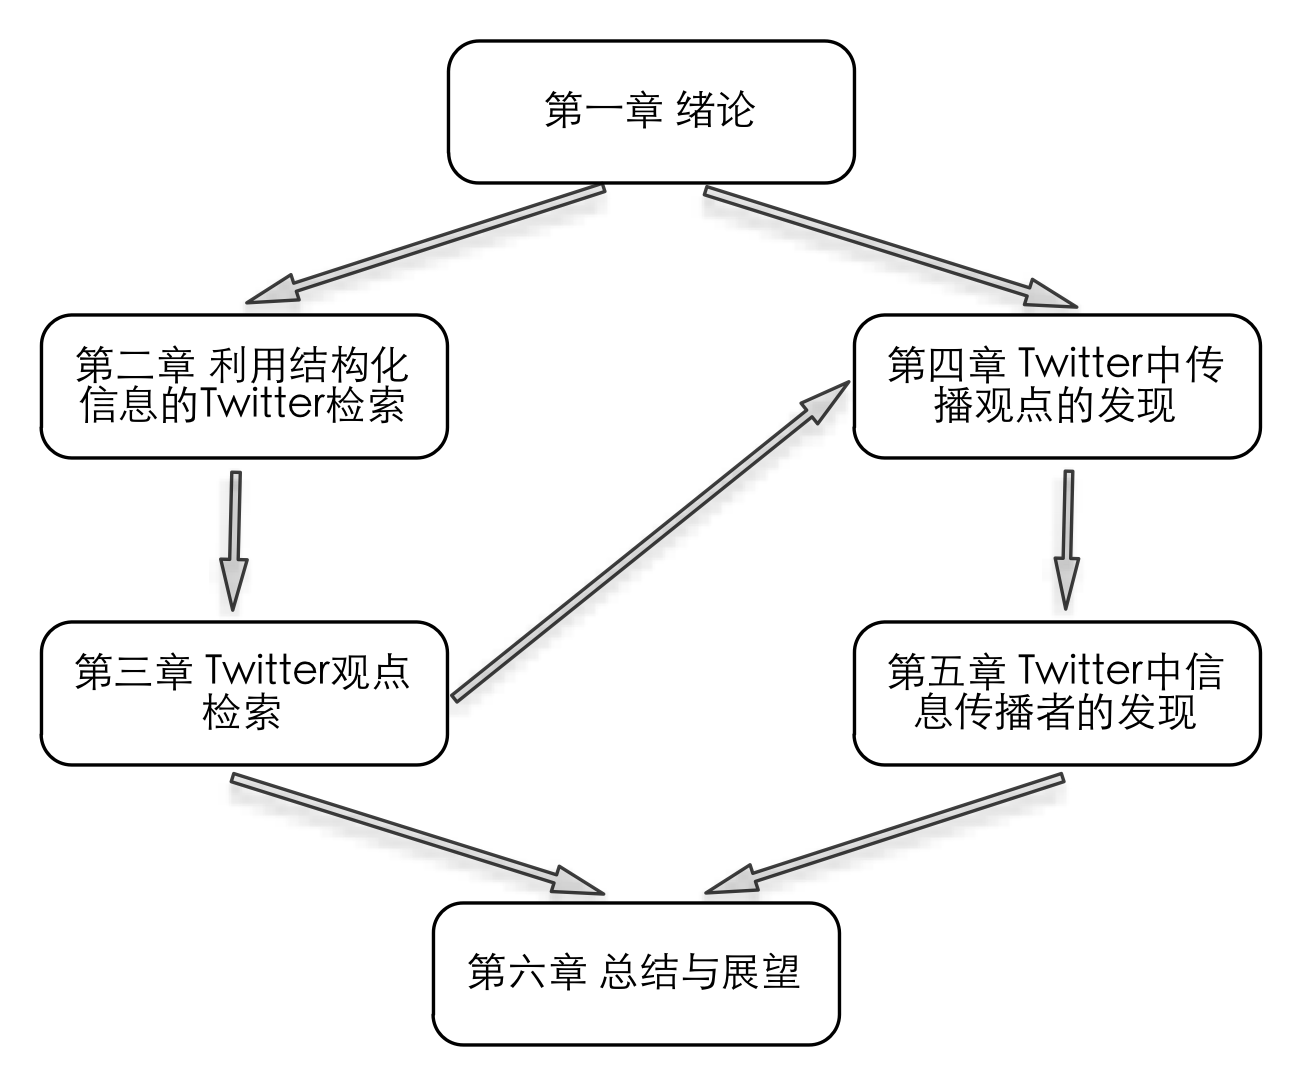
\includegraphics[height=250pt]{Paper_Framwork.png}
\caption{论文整体结构图}
\label{Paper_Framwork}
\end{figure}

第一章是绪论,首先介绍了本文研究的背景,介绍了社交媒体和Twitter的一些基础知识,接着提出研究动机,阐明了本文所涉及的科学问题、研究内容,并给出了研究方法,然后分析了研究问题,确立了依托自然语言处理技术与机器学习方法解决这些问题的基本思路,最后介绍了本文的主要工作和文章的结构。

第二章是Twitter中的信息检索,首先介绍了Twitter信息检索的研究背景,然后提出了以往Twitter信息检索方法忽视tweet文本结构化特点以及存在大量社交媒体信息的问题,以此设计了一种标注tweet文本结构的自动标注器,最后利用自动标注器标注tweet文本开发结构特征,结合社交媒体特征帮助Twitter信息检索,实验验证了方法的有效性。这一章回答了Twitter中
人们是如何用自然语言描述客观话题,并且社交媒体特征与tweet话题相关性存在怎样的联系。

第三章是Twitter中的观点检索,本章开头定义了Twitter中的观点检索问题,分析了Twitter观点检索与以往观点检索的不同特点,接着提出了一种自动获取主观tweet与客观tweet的方法自动生成情感词典,依靠词典对tweet的文本进行主观化判定,结合tweet的用户属性信息和文本信息,利用排序学习算法,实现观点检索。实验部分,我们构造了自己的Twitter观点检索语料,并发布了语料供以后的研究者使用,实验结果证明了我们的观点检索方法有效。这一章回答了Twitter中人们是如何用自然语言表达主观观点,并且社交媒体特征与tweet观点相关性存在怎样的联系。

第四章中我们针对Twitter观点检索存在大量低质量观点的问题,依据转发tweet一般是高质量文本的既有研究成果,提出了在Twitter中发现传播观点的问题。我们首先定义了问题,然后构造了数据集,接着开发了tweet传播度特征、观点化特征和文本质量特征,将其整合到排序学习的机器学习模型框架中。实验结果说明了这些特征对于Twitter中发现传播观点是有帮助的,另外我们的方法可以达到人判定传播观点的效果。这一章回答了Twitter中人们是如何用自然语言表达传播性的观点,并且社交媒体特征与传播性的观点存在怎样的联系。

第五章中我们探讨了Twitter中发现信息传播者的问题,给定一个tweet,发现tweet的作者粉丝中谁会转发该消息。我们开发了转发历史特征 、用户特征、用户活跃时间特征和用户兴趣特征,并依然将其应用到排序学习的框架中构造模型进行排序。实验部分,我们构造了自己的测试数据与基准系统,我们公布了数据,实验结果显示了我们的方法能够成功找到tweet转发者。这一章回答了社交媒体特征与信息传播者存在怎样的联系。

最后一章是总结部分,我们阐明了本文工作的贡献点,并且指出了工作的一些不足,并对未来社交媒体检索与传播分析的一些问题和方法进行了尝试性地思考。


